%\section{Proposed Model}
\section{Proposed Model} 
We will use Deep Learning or FCNNs in our work which is a Black-Box function. Generally, Black boxes work excellently but their structure won’t give you any insights that will explain how the function is being approximated. For this, we will use LIME as It is regarded as the most well-known XAI related python libraries. There are a lot of XAI frameworks that explain the Black-Box model’s insights by features. XAI functions work well in terms of explaining complex classification models. In short, these functions generate an explanation through charts of graphs for a complex model’s prediction which are also pretty fast. In Figure 4.1 we will see how black boxes work.

\vspace{5mm}
\begin{figure}[htbp]
\centering
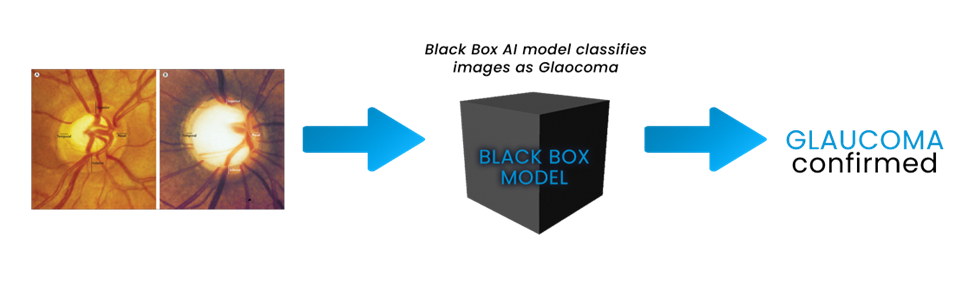
\includegraphics[scale=0.70]{images/fig-1.png}
\caption{Blackbox models confirming glaucoma through images}
\label{fig:x Blackbox models confirming glaucoma through images}
\end{figure}

\vspace{5mm}
In Figure 4.2 we will see how black boxes actually work with the help of lime.

\vspace{5mm}
\begin{figure}[htbp]
\centering
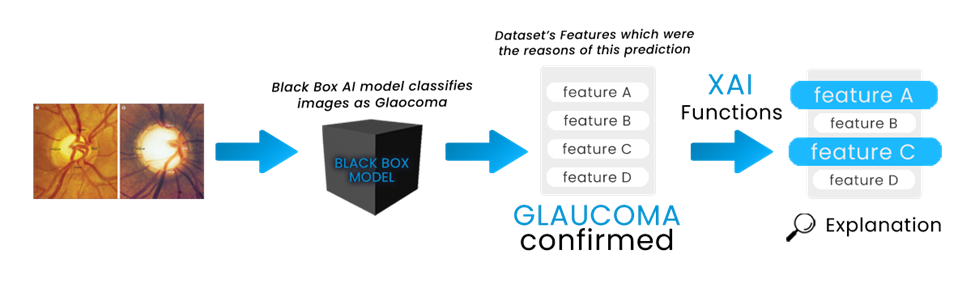
\includegraphics[scale=0.70]{images/fig-2.png}
\caption{Blackbox models decision making explanation through LIME}
\label{fig:x Blackbox models decision making explanation through LIME}
\end{figure}

\vspace{5mm}
\noindent Here we can see BlackBox models generate a result or output based on some features from the given/training datasets. And through lime, we can have a visualization from which features the output was based on.

\vspace{5mm}
\noindent In our Glaucoma dataset, we have some features for Suspicious glaucoma and Non-glaucoma. In both sections, we have fundus images, and labels as 1 as the confirmed glaucoma case and 0 as the Non-glaucoma case. To apply XAI, we took Fully Connected Neural Networks (FCNNs) as a black box AI model to predict glaucoma with the help of the data. To compile all of these classifications and determine the average of these scores to one single output, as in convolutional layers, we are using the ReLU nonlinear activation function and in the output nodes we are using the Softmax activation function. Below a short rendition is being given for the above Deep Learning models.

\vspace{5mm}
\noindent \textbf{1. Convolutional Neural Network (CNN)}: A convolutional neural network (CNN) is a type of deep neural network that is most typically used to evaluate visual images in deep learning. We will classify the image data through this model.

\vspace{5mm}
\noindent \textbf{2. Fully Connected Neural Network (FCNNs)}: FCNNs are a sort of artificial neural network in which all nodes, or neurons, in one layer are linked to neurons in the following layers [22]. FCNN model will also help us to predict and output.

\vspace{5mm}
\noindent \textbf{3. ReLU}: The activation function is implemented using a rectified linear activation unit, or ReLU for shorthand. Rectified networks are sometimes referred to as networks with hidden layers that employ this rectifier function. The computational cost of adding more ReLUs increases linearly as the size of the CNN grows.

\vspace{5mm}
\noindent \textbf{4. Softmax}:  that converts an integer vector into a probabilities vector, with the likelihood of each value proportional to the vector's relative scale is called softmax.  This model is programmed to generate N values, one for each classification task class, and the softmax function is used to normalize the outputs, converting these form weighted sum values to probabilities that add to just one. It is used for multi-classification in a logistic regression model, used in output layers for those networks that classify the inputs into multiple groups. This will compile all the convolutional layers of the FCNNs into a single output.

\newpage
\section{Work Plan} 
According to our Dataset, we will divide the data chronologically into training and testing data to classify glaucoma.. And through Lime, a XAI function, we will explain these black boxes.

\begin{figure}[htbp]
\centering
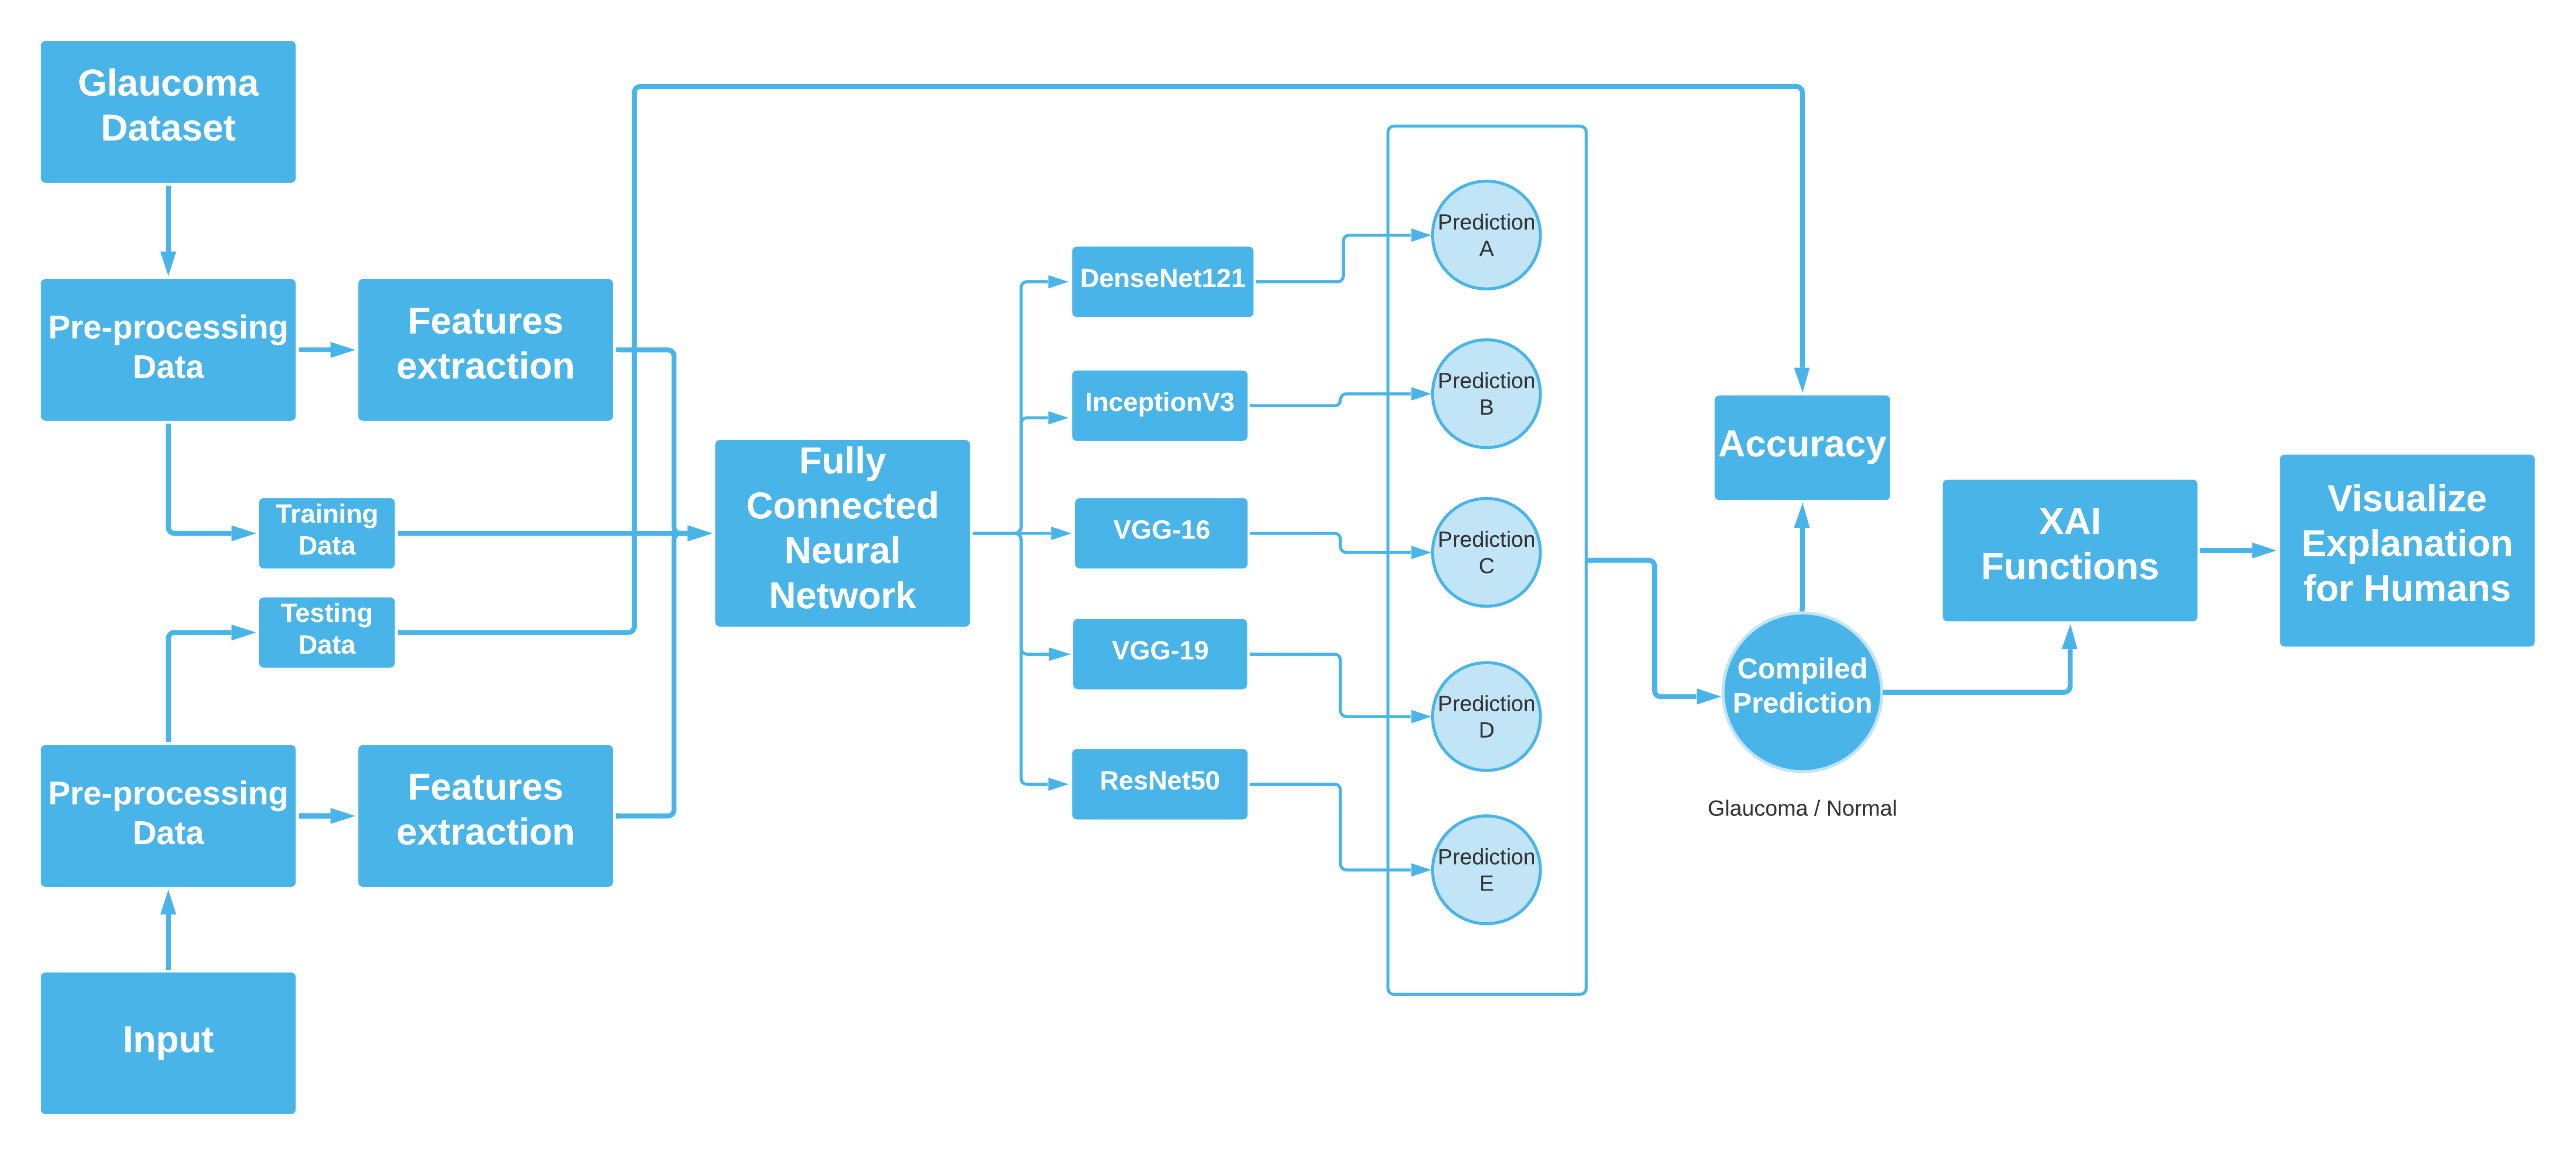
\includegraphics[scale=0.08]{images/work plan.png}
\caption{Work plan of the whole project}
\label{fig:x Work plan of the whole project}
\end{figure}

\vspace{5mm}
\noindent Here in [Figure 4.3], we have shown the whole process from dataset preprocessing to compiled output through Softmax activation function. And with XAI functions, we will explain the black boxes through visualization charts of the used core features which were the main reasons behind the prediction.

\vspace{5mm}
\noindent In our glaucoma dataset, we have some features for suspicious glaucoma and non-suspicious glaucoma. However, data visualization methods aim to produce more transparent and explainable decisions. In addition, CNN Based models are visually explainable for decision making and have gained significant attention in image classification [4]. A few works focus on preparing a Convolution Neural Network (CNN) by brute force while others use division and element extraction methods to identify glaucoma [5]. To apply for XAI we took Conventional Neural Network (CNN) architecture with fully connected layers or in other words Fully Connected Neural Network (FCNN). XAI frameworks LIME has been used for building trust among humans about the decisions made by AI models which are possibly making the black box models more transparent. Moreover, working with these AI models is not understandable by the common man and professionals. Additionally, AI and Machine Learning are essential for building trust among humans for decision making which is only possible by making black-box models more transparent through Explainable AI Frameworks which tries to explain their working.